
%(BEGIN_QUESTION)
% Copyright 2011, Tony R. Kuphaldt, released under the Creative Commons Attribution License (v 1.0)
% This means you may do almost anything with this work of mine, so long as you give me proper credit

Connect an ``ice cube'' relay to one of the outputs on a PLC, so that the PLC can control the energization of the relay.  All electrical connections must be made using a terminal strip (no twisted wires, crimp splices, wire nuts, spring clips, or ``alligator'' clips permitted).  Program this PLC to implement a motor start/stop (latching) control function.  {\it In order to ensure your program has not been pre-written in your computer prior to this assessment, you will be asked to sketch a correct ladder-diagram PLC program on paper to implement this function prior to using a computer.}

You must connect a ``commutating'' diode in parallel with the relay's coil to prevent the phenomenon known as ``inductive kickback,'' which may otherwise damage the transistor output on a PLC.  Note that incorrectly connecting this diode will present a short-circuit to the PLC, so you {\it must} get it right!

This exercise tests your ability to properly interpret the ``pinout'' of an electromechanical relay, properly wire a PLC output channel to control a relay's coil, properly polarize a commutating diode to prevent inductive kickback from damaging the PLC output, and use a terminal strip to organize all electrical connections.  It also tests your ability to program motor start/stop logic using either a seal-in contact or latching (retentive) coil instructions.

$$\includegraphics[width=15.5cm]{i00127x01.eps}$$

\vskip 10pt

The following components and materials will be available to you: assorted ``ice cube'' {\bf relays} with DC-rated coils and matching {\bf sockets} ; {\bf terminal strips} ; 1N400X rectifying {\bf diodes} ; lengths of {\bf hook-up wire}.  You will be expected to supply your own screwdrivers and multimeter for assembling and testing the circuit at your desk.  

\vskip 20pt

\noindent
{\bf ``Start'' switch to input}: \underbar{\hskip 20pt} \hskip 30pt {\bf ``Stop'' switch to input}: \underbar{\hskip 20pt} \hskip 30pt {\bf Relay to output}: \underbar{\hskip 20pt}

\vskip 20pt

\noindent
{\bf PLC program} (instructor chooses): \hskip 20pt \underbar{\hskip 20pt} Seal-in contact \hskip 20pt \underbar{\hskip 20pt} Retentive coils



\vfil

\underbar{file i00127}
\eject
%(END_QUESTION)





%(BEGIN_ANSWER)


%(END_ANSWER)





%(BEGIN_NOTES)


%INDEX% Mastery exam performance exercise (circuit), drive a relay coil with a PLC output

%(END_NOTES)


